\documentclass[journal]{IEEEtran}

% *** CITATION PACKAGES ***
\usepackage{cite}

% *** GRAPHICS RELATED PACKAGES ***
%
\ifCLASSINFOpdf
\usepackage[pdftex]{graphicx}
  % declare the path(s) where your graphic files are
  % \graphicspath{{../pdf/}{../jpeg/}}
  % and their extensions so you won't have to specify these with
  % every instance of \includegraphics
  % \DeclareGraphicsExtensions{.pdf,.jpeg,.png}
\else
  % or other class option (dvipsone, dvipdf, if not using dvips). graphicx
  % will default to the driver specified in the system graphics.cfg if no
  % driver is specified.
  % \usepackage[dvips]{graphicx}
  % declare the path(s) where your graphic files are
  % \graphicspath{{../eps/}}
  % and their extensions so you won't have to specify these with
  % every instance of \includegraphics
  % \DeclareGraphicsExtensions{.eps}
\fi
% graphicx was written by David Carlisle and Sebastian Rahtz. It is
% required if you want graphics, photos, etc. graphicx.sty is already
% installed on most LaTeX systems. The latest version and documentation
% can be obtained at: 
% http://www.ctan.org/pkg/graphicx
% Another good source of documentation is "Using Imported Graphics in
% LaTeX2e" by Keith Reckdahl which can be found at:
% http://www.ctan.org/pkg/epslatex
%
% latex, and pdflatex in dvi mode, support graphics in encapsulated
% postscript (.eps) format. pdflatex in pdf mode supports graphics
% in .pdf, .jpeg, .png and .mps (metapost) formats. Users should ensure
% that all non-photo figures use a vector format (.eps, .pdf, .mps) and
% not a bitmapped formats (.jpeg, .png). The IEEE frowns on bitmapped formats
% which can result in "jaggedy"/blurry rendering of lines and letters as
% well as large increases in file sizes.
%
% You can find documentation about the pdfTeX application at:
% http://www.tug.org/applications/pdftex






% *** PDF, URL AND HYPERLINK PACKAGES ***
%
%\usepackage{url}
% url.sty was written by Donald Arseneau. It provides better support for
% handling and breaking URLs. url.sty is already installed on most LaTeX
% systems. The latest version and documentation can be obtained at:
% http://www.ctan.org/pkg/url
% Basically, \url{my_url_here}.


% correct bad hyphenation here
\hyphenation{op-tical net-works semi-conduc-tor}


\begin{document}
%
% paper title
% Titles are generally capitalized except for words such as a, an, and, as,
% at, but, by, for, in, nor, of, on, or, the, to and up, which are usually
% not capitalized unless they are the first or last word of the title.
% Linebreaks \\ can be used within to get better formatting as desired.
% Do not put math or special symbols in the title.
\title{Detección de Fracturas en Radiografías Mediante Transfer Learning}


\author{Álvaro Salgado López}

% note the % following the last \IEEEmembership and also \thanks - 
% these prevent an unwanted space from occurring between the last author name
% and the end of the author line. i.e., if you had this:
% 
% \author{....lastname \thanks{...} \thanks{...} }
%                     ^------------^------------^----Do not want these spaces!
%
% a space would be appended to the last name and could cause every name on that
% line to be shifted left slightly. This is one of those "LaTeX things". For
% instance, "\textbf{A} \textbf{B}" will typeset as "A B" not "AB". To get
% "AB" then you have to do: "\textbf{A}\textbf{B}"
% \thanks is no different in this regard, so shield the last } of each \thanks
% that ends a line with a % and do not let a space in before the next \thanks.
% Spaces after \IEEEmembership other than the last one are OK (and needed) as
% you are supposed to have spaces between the names. For what it is worth,
% this is a minor point as most people would not even notice if the said evil
% space somehow managed to creep in.








% If you want to put a publisher's ID mark on the page you can do it like
% this:
%\IEEEpubid{0000--0000/00\$00.00~\copyright~2015 IEEE}
% Remember, if you use this you must call \IEEEpubidadjcol in the second
% column for its text to clear the IEEEpubid mark.



% use for special paper notices
%\IEEEspecialpapernotice{(Invited Paper)}


\markboth{Procesamiento Y Clasificación de Datos, 20 Febrero 2025}{}

% make the title area
\maketitle



%\IEEEpeerreviewmaketitle



\section{Introducción}
% The very first letter is a 2 line initial drop letter followed
% by the rest of the first word in caps.
% 
% form to use if the first word consists of a single letter:
% \IEEEPARstart{A}{demo} file is ....
% 
% form to use if you need the single drop letter followed by
% normal text (unknown if ever used by the IEEE):
% \IEEEPARstart{A}{}demo file is ....
% 
% Some journals put the first two words in caps:
% \IEEEPARstart{T}{his demo} file is ....
% 
% Here we have the typical use of a "T" for an initial drop letter
% and "HIS" in caps to complete the first word.
\IEEEPARstart
{L}{a} detección de fracturas en radiografías es una tarea crucial en el diagnóstico médico, ya que permite una identificación temprana y precisa de lesiones óseas, facilitando el tratamiento adecuado para los pacientes. Sin embargo, la evaluación manual de estas imágenes requiere de un alto grado de experiencia por parte de los especialistas y está sujeta a errores humanos. En este contexto, la aplicación de algoritmos de aprendizaje profundo, en particular las redes neuronales convolucionales (CNNs), ha demostrado ser una solución eficiente para la automatización del proceso de clasificación y detección de anomalías en imágenes médicas.

El presente estudio tiene como objetivo el diseño e implementación de un modelo basado en la arquitectura VGG16, utilizando técnicas de $transfer learning$ y $fine-tuning$, para clasificar radiografías en dos categorías: con fractura y sin fractura. Esta metodología se justifica por el excelente desempeño reportado por modelos preentrenados en tareas de reconocimiento de patrones en imágenes médicas.
% You must have at least 2 lines in the paragraph with the drop letter
% (should never be an issue)

\section{Metodología}
El conjunto de datos empleado en este estudio fue obtenido de $Kaggle$ y está compuesto por radiografías clasificadas en dos grupos: imágenes de huesos fracturados y no fracturados, tanto para entrenamiento como para validación se aplicó un $ImageDataGenerator$ para normalizar y aumentar artificialmente la cantidad de imágenes, generando variaciones en iluminación, rotaciones y escalados.

\subsection{Arquitectura del Modelo}
Se seleccionó la arquitectura VGG16 preentrenada con pesos de $ImageNet$ debido a su eficacia en tareas de clasificación de imágenes. Se llevaron a cabo las siguientes modificaciones:

Se eliminaron las capas superiores del modelo original y se añadió una nueva capa completamente conectada con activación sigmoide para la clasificación binaria.

Se congelaron las primeras capas convolucionales para emplear $transfer learning$, permitiendo que el modelo aproveche las representaciones aprendidas previamente.

Se realizó $fine-tuning$ sobre las capas superiores del modelo con el objetivo de adaptar las representaciones a las características específicas de las radiografías.

\subsection{Entrenamiento}
El modelo se entrenó empleando la siguiente configuración:
\begin{itemize}
    \item Optimizador: Adam con una tasa de aprendizaje inicial de 1e-4, ajustada de manera dinámica mediante reducción de la tasa de aprendizaje en caso de estancamiento en la validación.
    \item Función de pérdida: $Binary Crossentropy$, adecuada para problemas de clasificación binaria.
    \item Estrategias de regularización: Se utilizó $Dropout$ para reducir el riesgo de sobreajuste y $Early Stopping$ para detener el entrenamiento cuando no se observaba mejora significativa en la validación.
\end{itemize}

El modelo fue entrenado durante múltiples épocas y se seleccionaron los pesos óptimos en función del mejor desempeño en el conjunto de validación.


\section{Resultados}
Para evaluar el desempeño del modelo de clasificación basado en VGG16, se analizaron diversas métricas sobre el conjunto de datos de validación. En esta sección, se presentan los resultados obtenidos en términos de exactitud, junto con una interpretación detallada de la matriz de confusión. Estos análisis permiten identificar las fortalezas y limitaciones del modelo en la detección de fracturas en imágenes de rayos X, así como posibles estrategias para mejorar su desempeño.
\begin{figure}
    \centering
    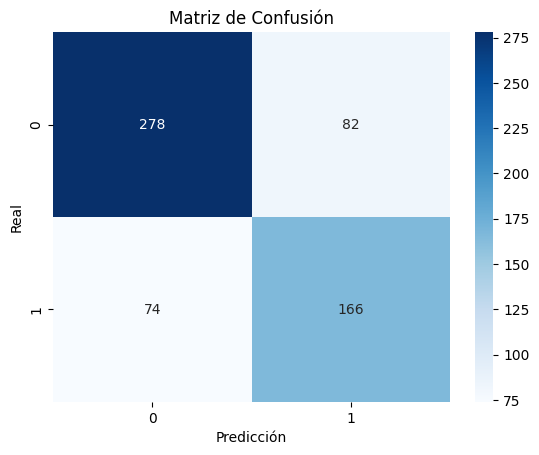
\includegraphics[width=0.9\linewidth]{Figs/CM.png}
    \caption{Matriz de confusión en el conjunto de validación}
    \label{CM}
\end{figure}

En la Fig \ref{CM} se aprecia que el modelo tiene un mejor desempeño en la detección de imágenes sin fractura que en la identificación de fracturas. Esto se evidencia en la mayor cantidad de falsos negativos (74), lo que implica que hay fracturas que el modelo no está detectando. 

La precisión general del modelo alcanzó un 74\%, lo que indica un desempeño moderado. Aunque esta cifra es aceptable en un problema de clasificación binaria en imágenes médicas, un rendimiento superior es deseable debido a la importancia clínica del diagnóstico.

\begin{figure}
    \centering
    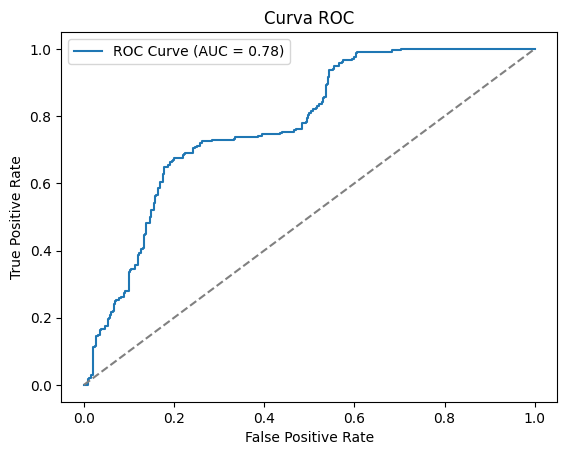
\includegraphics[width=0.9\linewidth]{Figs/ROC.png}
    \caption{Curva ROC}
    \label{ROC}
\end{figure}

En la Fig \ref{ROC} se observa la curva ROC obtenida, ésta muestra una capacidad moderada del modelo para distinguir entre imágenes con y sin fractura, con un área bajo la curva (AUC) de 0.78. Este valor indica que el modelo es significativamente mejor que un clasificador aleatorio, pero aún tiene margen de mejora.

En el contexto de la detección de fracturas, donde la precisión del diagnóstico es crítica, un AUC de 0.78 sugiere que el modelo puede diferenciar correctamente en la mayoría de los casos, aunque todavía presenta limitaciones. Si bien logra identificar una buena proporción de fracturas, el hecho de que no se aproxime a valores superiores a 0.85 indica que existen casos en los que puede generar falsos positivos o falsos negativos de manera significativa.

Dado que los falsos negativos pueden implicar riesgos clínicos considerables al no detectar fracturas reales, es importante considerar estrategias para mejorar la sensibilidad del modelo sin comprometer en exceso la especificidad. Algunas opciones incluyen un ajuste más profundo de los hiperparámetros, la aplicación de técnicas de preprocesamiento enfocadas en resaltar las estructuras óseas o la incorporación de arquitecturas más avanzadas. En general, si bien el desempeño del modelo es adecuado para un primer enfoque, es recomendable seguir optimizando su precisión antes de su posible implementación en un entorno clínico real.
\section{Conclusión}
El modelo basado en VGG16 mostró un desempeño aceptable en la clasificación de fracturas en radiografías, con una precisión global del 74\% y un AUC de 0.78 en la curva ROC. Estos resultados indican que el modelo es capaz de diferenciar entre imágenes con y sin fractura en la mayoría de los casos, pero aún presenta limitaciones que podrían comprometer su aplicabilidad en un entorno clínico.

Si bien la detección de fracturas es adecuada en términos generales, el modelo tiene un desempeño desigual entre clases, mostrando mejor precisión para la categoría “No Fractura” en comparación con “Fractura”. Esto sugiere que el modelo puede estar sesgado hacia la detección de imágenes sin fracturas, lo que podría derivar en falsos negativos con consecuencias potencialmente graves en un contexto médico.

Para mejorar el rendimiento, sería recomendable aplicar técnicas de aumento de datos enfocadas en mejorar la representación de fracturas, ajustar aún más las capas intermedias del modelo mediante $fine-tuning$. También se podría considerar el uso de enfoques híbridos con métodos de interpretación de imágenes médicas, como $Grad-CAM$, para mejorar la comprensión de las decisiones del modelo.

En conclusión, aunque el modelo representa un avance prometedor en la clasificación automatizada de fracturas en radiografías, se requieren mejoras adicionales para garantizar una precisión diagnóstica confiable antes de su implementación en entornos clínicos reales.
% Can use something like this to put references on a page
% by themselves when using endfloat and the captionsoff option.
\ifCLASSOPTIONcaptionsoff
  \newpage
\fi



% trigger a \newpage just before the given reference
% number - used to balance the columns on the last page
% adjust value as needed - may need to be readjusted if
% the document is modified later
%\IEEEtriggeratref{8}
% The "triggered" command can be changed if desired:
%\IEEEtriggercmd{\enlargethispage{-5in}}

% references section

% can use a bibliography generated by BibTeX as a .bbl file
% BibTeX documentation can be easily obtained at:
% http://mirror.ctan.org/biblio/bibtex/contrib/doc/
% The IEEEtran BibTeX style support page is at:
% http://www.michaelshell.org/tex/ieeetran/bibtex/
%\bibliographystyle{IEEEtran}
% argument is your BibTeX string definitions and bibliography database(s)
%\bibliography{IEEEabrv,../bib/paper}
%
% <OR> manually copy in the resultant .bbl file
% set second argument of \begin to the number of references
% (used to reserve space for the reference number labels box)

%\bibliographystyle{IEEEtran} % Estilo de citas de IEEE
%\bibliography{referencias} % Nombre de tu archivo .bib


\end{document}


